\begin{frame}{Secret Sharing $L_\infty$ ball}
    \begin{itemize}
        \item For center $(x_1, \ldots, x_d)$, we want to secret share this huge $L_\infty$ ball:
        \begin{equation*}
            [x_1 - \delta, x_1 + \delta] \times [x_2 - \delta, x_2 + \delta] \times \ldots \times [x_n - \delta, x_n + \delta]
        \end{equation*}

        \only<2>{
        \item We can secret share each dimension separately, then AND the results.
        \begin{equation*}
            y_1 \ge x_1 - \delta \quad \wedge \quad y_1 \le x_1 + \delta \quad \wedge \quad \ldots \quad \wedge \quad y_d \ge x_d - \delta \quad \wedge \quad y_d \le x_d + \delta
        \end{equation*}
        }

    \end{itemize}

    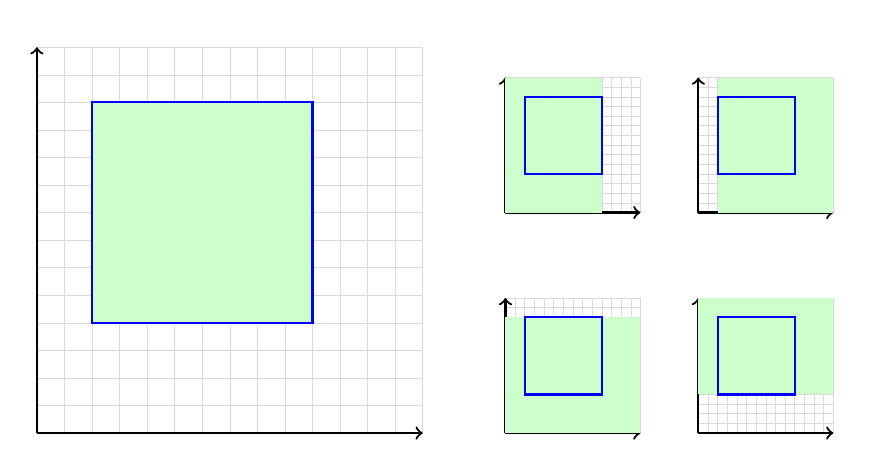
\begin{tikzpicture}[scale=0.7]
        % light grid
        \draw[step=0.5cm,gray!30,very thin] (0, 0) grid (7, 7);
    
        % axes
        \draw[->,thick] (0,0) -- (7,0) node[right] {};
        \draw[->,thick] (0,0) -- (0,7) node[above] {};
    
        % square with corners (1,2) and (5,6)
        \draw[thick,blue,fill=green!20] (1,2) rectangle (5,6);
    
        % optional: mark the corners
        % \filldraw[blue] (1,2) circle (2pt);
        % \filldraw[blue] (5,6) circle (2pt);
    
        % small planes on the right (2x2)
        \only<2>{
        \begin{scope}[xshift=8.5cm,yshift=4cm,scale=0.35]
            \draw[step=0.5cm,gray!30,very thin] (0, 0) grid (7, 7);
            \draw[->,thick] (0,0) -- (7,0) node[right] {};
            \draw[->,thick] (0,0) -- (0,7) node[above] {};
            \fill[green!20] (0,0) rectangle (5,7);
            \draw[thick,blue] (1,2) rectangle (5,6);
        \end{scope}
        \begin{scope}[xshift=12cm,yshift=4cm,scale=0.35]
            \draw[step=0.5cm,gray!30,very thin] (0, 0) grid (7, 7);
            \draw[->,thick] (0,0) -- (7,0) node[right] {};
            \draw[->,thick] (0,0) -- (0,7) node[above] {};
            \fill[green!20] (1,0) rectangle (7,7);
            \draw[thick,blue] (1,2) rectangle (5,6);
        \end{scope}
        \begin{scope}[xshift=8.5cm,yshift=0cm,scale=0.35]
            \draw[step=0.5cm,gray!30,very thin] (0, 0) grid (7, 7);
            \draw[->,thick] (0,0) -- (7,0) node[right] {};
            \draw[->,thick] (0,0) -- (0,7) node[above] {};
            \fill[green!20] (0,0) rectangle (7,6);
            \draw[thick,blue] (1,2) rectangle (5,6);
        \end{scope}
        \begin{scope}[xshift=12cm,yshift=0cm,scale=0.35]
            \draw[step=0.5cm,gray!30,very thin] (0, 0) grid (7, 7);
            \draw[->,thick] (0,0) -- (7,0) node[right] {};
            \draw[->,thick] (0,0) -- (0,7) node[above] {};
            \fill[green!20] (0,2) rectangle (7,7);
            \draw[thick,blue] (1,2) rectangle (5,6);
        \end{scope}
        }
    \end{tikzpicture}

\end{frame}
% Note: In the script, state clearly that in this talk to keep things simple, we do not talk about overflow

\begin{frame}
    \frametitle{Primitive: Function Secret Sharing (FSS)}
    \begin{itemize}
        \item FSS was introduced in \cite{boyle2015function}, allowing to secret share a function $f$ between multiple parties.
        \item For domain bit length $u$, security parameter $\kappa$, payload bit length $v$, the key size is $O(u \cdot (\kappa + v))$ bits.
    \end{itemize}
    \begin{center}
    \begin{tikzpicture}[>=stealth,thick]
        \node[minimum width=1.5cm,minimum height=1.2cm,align=center] (interval) at (0,0) {$x \le a?$};
        \node (oracle) at (2,0) {\includegraphics[width=2.6cm]{images/crystal_ball_transparent.png}};
        \node (key1) at (8,1.4) {\includegraphics[width=1.8cm]{images/key_transparent.png}};
        \node (key0) at (8,-1.4) {\includegraphics[width=1.8cm]{images/key_transparent.png}};

        \draw[->] (interval.east) -- (oracle.west);
        \draw[->] (oracle.east) -- (key1.west);
        \draw[->] (oracle.east) -- (key0.west);

        \node at ([yshift=0pt]key1.north) {$k_1$};
        \node at ([yshift=0pt]key0.south) {$k_0$};
    \end{tikzpicture}
    \end{center}
\end{frame}

\begin{frame}
    \frametitle{Function Secret Sharing in \cite{garimella2024computation}}
    \begin{itemize}
        \item Alice prepares $O(\kappa)$ FSS keys pairs with \textit{binary output} (\textit{in} / \textit{out}?) for each dimension.
    \end{itemize}
    \begin{center}
    \begin{tikzpicture}[>=stealth,thick,node distance=0.8cm and 1.1cm,xscale=0.9]
        \node[anchor=north west] (alice) at (-0.5,2.6) {\includegraphics[height=1.6cm]{images/Alice_transparent.png}};

        \node (t1) at (0,0) {$y_1 \ge x_1 - \delta$};
        \node (t2) [right=1.4cm of t1] {$y_1 \le x_1 + \delta$};
        \node (dots) [right=1.0cm of t2] {$\cdots$};
        \node (td) [right=1.0cm of dots] {$y_d \le x_d + \delta$};

        \foreach \i/\src in {1/t1,2/t2,3/td} {
            \node (k0\i) [below left=0.7cm and 0.2cm of \src] {$k_0^{\i}$};
            \node (k1\i) [below right=0.7cm and 0.2cm of \src] {$k_1^{\i}$};
            \draw[->] (\src.south west) -- (k0\i.north);
            \draw[->] (\src.south east) -- (k1\i.north);
        }
    \end{tikzpicture}
    \end{center}
\end{frame}

\begin{frame}
    \frametitle{Why do we need $\kappa$ key pair?}
\end{frame}